\chapter{Contexto Tecnológico}
\label{chap:contexto_tecnologico}

En este capítulo hacemos una introducción a algunos conceptos de la computación autónoma y los bucles de control. Son los conceptos principales en los que se basa el trabajo. Presentaremos la arquitectura MAPE-K, en la que se basa el sistema existente. También describiremos algunos conceptos de arquitecturas de \foreign{english}{software} que nos serán de interés.

\section{Computación autónoma y bucles de control}

Según \cite{ibmcorporationArchitecturalBlueprintAutonomic2006}, la \textbf{computación autónoma} tiene como objetivo dotar a los sistemas de \textbf{autonomía} en su operación. Es decir, capacidades para gestionarse a si mismos. Los sistemas deberán adaptarse a los cambios en su entorno de ejecución. Con esto, buscamos alcanzar una reducción en el coste de operación y hacer más manejable la complejidad de los sistemas.

Las adaptaciones pueden tomar distintas formas: cambios en sus parámetros de configuración, habilitar o deshabilitar funcionalidades, etc. Estas se realizan en base a directivas de alto nivel, los \textbf{ objetivos}. Un operario humano define las metas que el sistema debe alcanzar, y este intentará planificar acciones correctivas para alcanzarlo.

En base a estos parámetros, el sistema puede intuir que debe reconfigurarse para cumplir con los objetivos de operación que tiene mercados. Para ello, en base a una serie de estrategias predefinidas, es capaz de elegir su siguiente configuración. \cite{garlanIncreasingSystemDependability2003}. Esto conlleva mover a tiempo de ejecución las decisiones de arquitectura y funcionalidad. Con ello, buscamos permitir un comportamiento dinámico del sistema. .

\textcolor{red}{Tambien el internet de las cosas \emph{citation needed}}

Siguiendo con el ejemplo de la tienda \foreign{english}{on-line}, el operario podría definir un umbral máximo de carga por cada instancia. Cuando se supere, el sistema podría decidir que se requiere una acción correctiva. Por ejemplo, esta acción podría consistir en desplegar nuevas instancias del servicio. Cuando la carga de los servicios baje, podrá optar por eliminarlas.

Para implementar estas capacidades de adaptación se recurre a la teoría de control y al \textbf{bucle de control} (o \emph{feedback loop}). \cite{brunEngineeringSelfAdaptiveSystems2009} Se trata de un proceso iterativo para la gestión de sistemas. A partir de información sobre el estado del sistema y su entorno, pauta acciones correctivas. Estas se basan en heurísticas definidas por los administradores del sistema. Puede dividirse en cuatro etapas (figura \ref{fig:bucle-control}):

\begin{figure}[h]
  \centering
  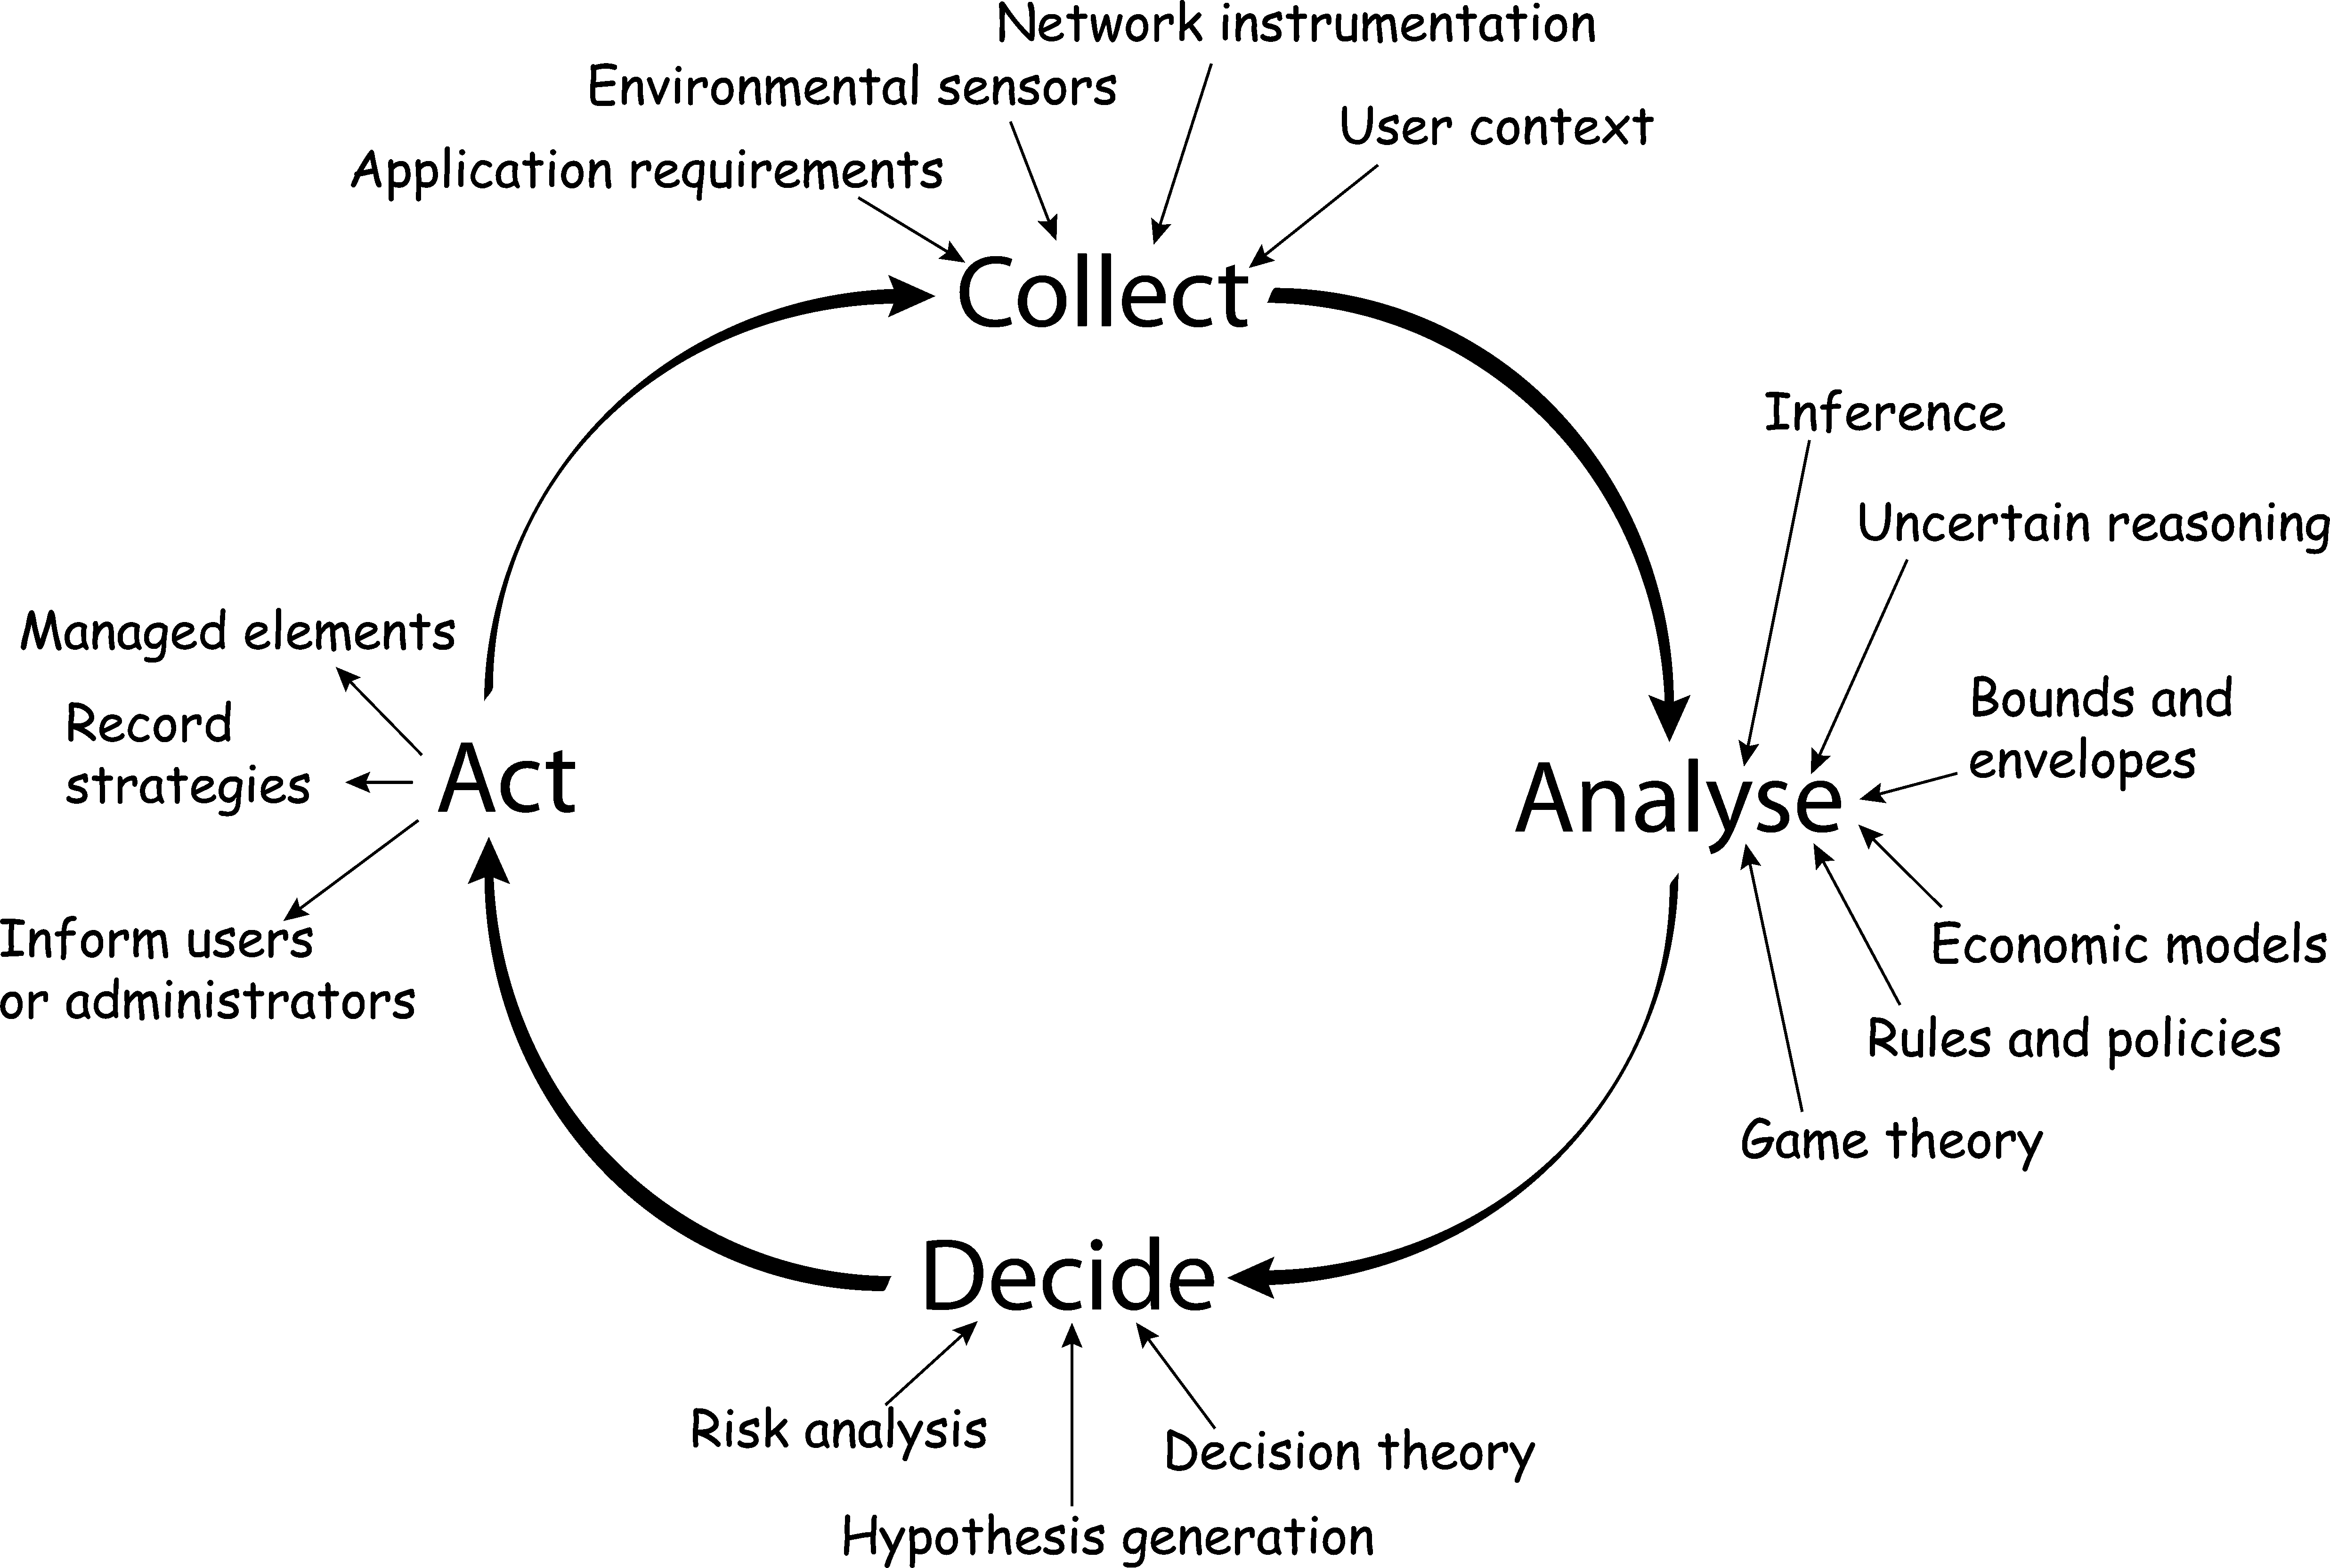
\includegraphics[scale=0.065]{cap_introduccion/images/feedback-loop}
  \caption[Un bucle de control genérico. Consta de cuatro actividades: Recopilar información, analizarla, decidir y actuar si procede.]{Un bucle de control genérico. Consta de cuatro actividades: Recopilar información, analizarla, decidir y actuar si procede. Obtenida de \cite{dobsonSurveyAutonomicCommunications2006}.}
  \label{fig:bucle-control}
\end{figure}

\begin{itemize}
  \item \textbf{Recopilar información}: El bucle \textbf{monitoriza} el estado del sistema a través de \textbf{sondas}. Estas reportan información del sistema y del entorno de ejecución. Pueden ser métricas de rendimiento, estado de los componentes, cambios en en el entorno, etc.

  Estos datos en bruto deben ser limpiados, filtrados y agregados para sintetizarlos en propiedades de nuestro interés. Si se considera que son relevantes, se almacenan para informar las siguientes etapas del bucle.

  \item \textbf{Analizar}: Basándose en la información considerada de interés, la etapa de análisis debe identificar \textbf{síntomas}: indicadores de una situación que requiera de nuestra atención. Puede ser mediante heurísticas predefinidas, análisis estadístico u otros métodos. Un ejemplo de síntoma sería ''uso de CPU elevado'', ''número elevado de mensajes encolados en un sistema de mensajería'', etc.

  \item \textbf{Decidir}: \textcolor{red}{A partir de los síntomas, el bucle debe determinar si es necesario tomar alguna acción. Si detecta que no estamos cumpliendo los objetivos, o que puede mejorarse la configuración actual, .} \textbf{Planifica} qué acciones deben llevarse a cabo para que el sistema se adapte y alcance una configuración deseable. Por ejemplo, si hay muchos mensajes encolados, se podría solicitar el iniciar otra instancia del servicio que los consuma y procese en paralelo.

  \item \textbf{Actuar}: Si se ha planificado alguna acción, se intentará \textbf{ejecutar} en esta etapa final. Mediante \textbf{efectores} en el sistema, el bucle es capaz de modificar su configuración. Dependiendo del éxito de ejecución, la adaptación se lleva a cabo o no. Finalizada esta etapa, se vuelve a recopilar información y arranca de nuevo el proceso.
\end{itemize}


\textcolor{red}{Hablar de human in the loop: solicitamos la intervención del humano cuando no contamos con suficiente información para tomar una acción correctiva.}

Este tipo de proceso está presente en gran variedad de contextos como puede ser operación de plantas industriales, \cite{climentpenadesDissenyPrototipatSolucions2020a}  en procesos naturales, etc. \textcolor{red}{ampliar}

\textcolor{red}{Hablar de agentes autónomos como aplicación práctica. \cite{savaglioAgentbasedInternetThings2020}}

En la ingeniería de \emph{software}, encontramos los bucles de control en dos variantes distintas: bucles de control implícitos o explícitos. La más habitual es la primera: se encuentran implícitos en la implementación de los procesos del sistema. \cite{brunEngineeringSelfAdaptiveSystems2009} No son componentes externos dedicados.

Por otro lado, aproximaciones como las de \cite{garlanIncreasingSystemDependability2003} o \cite{ibmcorporationArchitecturalBlueprintAutonomic2006} optan por la segunda: bucles como componentes externos. Esto permite separar la funcionalidad de las capacidades de adaptación.  Al dividirse estas responsabilidades, se puede reducir la complejidad de la implementación. En este trabajo nos centraremos en esta segunda variante.

\section{Arquitecturas para sistemas autónomos: Bucles MAPE-K}
\label{sec:bucles-mapek}

%% TODO: Buscar sinonimos de sistema..

Un estilo arquitectónico muy representativo es el basado en bucles MAPE-K \cite{ibmcorporationArchitecturalBlueprintAutonomic2006, fonsServiciosAdaptivereadyPara2021} propuesto por IBM. Se trata de una referencia arquitectónica para desarrollar sistemas distribuidos autónomos. Nace con el objetivo hacer más manejable la complejidad de estos sistemas; y reducir sus costes de operación, requiriendo de la minima intervención humana.

Su componentes principales son los \textbf{elementos autónomos}. Cada uno de estos es capaz de autogestionarse, y colaborar en conjunto con el resto de elementos autónomos del sistema  para alcanzar los objetivos. \textcolor{red}{¿Agent based?} A su vez, estos pueden dividirse en dos partes: los recursos manejados y un manejador autónomo (el bucle de control).

Los \textbf{recursos manejados} son las unidades de funcionalidad. Puede ser cualquier tipo de recurso, \emph{hardware} o \emph{software}. Para dotarlos de capacidad de autoadaptación, los emparejamos con un \textbf{manejador autónomo}: el bucle de control. Gestiona al recurso en base a la información que recoge del entorno de ejecución y las políticas que guían su adaptación.

El bucle es de tipo externo, ya que es un componente distinto al que implementa la funcionalidad. Por tanto, el recurso debe implementar puntos de contacto (\textbf{\emph{touchpoints}}): interfaces que permitan obtener información de su estado (sondas) y cambiar su configuración (efectores).

Estos elementos autónomos se auto-gestionan en base a \textbf{políticas}: un conjunto de objetivos de alto nivel definidos por sus administradores. El sistema tratará de mantener su cumplimiento durante su ejecución. Para alcanzarlos, el manejador autónomo planifica cambios en la configuración del recurso manejado.

\subsection{Estructura del bucle MAPE-K}

En la figura \ref{fig:autonomic-element} mostramos una representación de un elemento autónomo. Distinguimos las dos partes principales: el manejador y el recurso. El manejador contacta con el recurso a través de sus sensores y efectores. Podemos apreciar los componentes que conforman el bucle, y que describimos a continuación: \cite{ibmcorporationArchitecturalBlueprintAutonomic2006}

\begin{figure}[h]
  \centering
  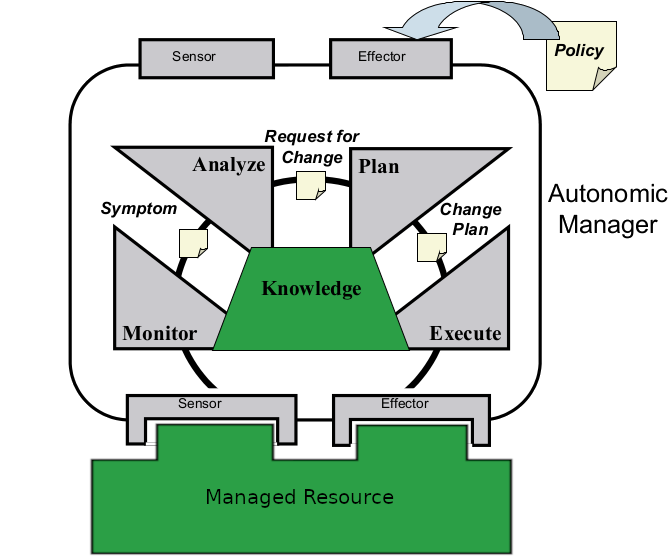
\includegraphics[scale=2]{cap_contexto_tecnologico/images/autonomic-element}
  \caption[Representación de un elemento autónomo. Distinguimos el recurso manejado y el manejador autónomo. El manejador es un bucle MAPE-K (\emph{Monitor}, \emph{Analysis}, \emph{Planification}, \emph{Execution} y \emph{Knowledge})]{Representación de un elemento autónomo. Distinguimos el recurso manejado y el manejador autónomo. El manejador es un bucle MAPE-K. Basada en imagen de \cite{ibmcorporationArchitecturalBlueprintAutonomic2006}.}
  \label{fig:autonomic-element}
\end{figure}

Para presentar estos componentes, describiremos un ejemplo de cómo se manejaría un servicio web. Nos centraremos en escalar este servicio en base a la carga del sistema. Deseamos que, en caso de carga elevada, se desplieguen nuevas instancias. Si la carga bajara, el sistema debería eliminar las instancias redundantes.

\subsubsection{Sondas}

Para monitorizar el recurso y su entorno debemos \textbf{instrumentarlos}. Consiste en implementar \textbf{sondas} que expongan datos relevantes a los monitores del bucle. Pueden capturar y transmitir cualquier aspecto que queramos controlar: \emph{health checks}, rendimiento del servicio u otras propiedades del sistema.

Para nuestro servicio web, una métrica relevante sería el número de peticiones por segundo que está atendiendo. La sonda reportaría el número de peticiones que se han atendido hasta un determinado momento.

\subsubsection{Monitor}

El monitor recibe las mediciones de las sondas. Se encarga de recogerlas, agregarlas y filtrarlas para extraer información relevante. La información se almacenará como propiedades de adaptación en la base de conocimiento.\cite{fonsEspecificacionSistemasAutoadaptativos2021} El monitor y las sondas componen la etapa de recopilar información de los bucles de control.

Siguiendo con nuestro ejemplo, el monitor recibiría el número de peticiones atendidas, y las agregaría en una métrica de serie temporal de peticiones por segundo. Esta sería una de nuestras propiedades de adaptación. En base a ella, las siguientes etapas tomarán las decisiones convenientes para escalar nuestro servicio.

\subsubsection{Base de conocimiento}

La base de conocimiento (\emph{knowledge base}) es el componente base de toda la arquitectura. Informa a todas las etapas del bucle de control. Por lo que se trata de un componente transversal. \textcolor{red}{Es una arquitectura knowledge-driven \cite{taylorSoftwareArchitectureFoundations2009}.}

Está compuesta por una o más fuentes de información que el bucle tiene a su disposición. A partir de ellas, se almacenan las \textbf{propiedades de adaptación}. Estas describen el estado pasado y presente del sistema y su entorno: métricas, componentes, conexiones entre ellos, parámetros de configuración\dots

En conjunto, estas propiedades conforman un modelo abstracto del estado del recurso manejado que se mantiene en tiempo de ejecución. \cite{garlanIncreasingSystemDependability2003}. Las demás etapas del bucle operan en base a él. Como veremos más adelante, los efectores se encargan de traducir las acciones correctivas del modelo de alto nivel a términos del recurso manejado.

\subsubsection{Analizador}

En base al modelo abstracto del sistema, podemos razonar sobre el estado actual sin acoplarnos al recurso manejado. Podemos definir heurísticas que nos permitan detectar situaciones que requieran de una acción correctiva. Esta es la función del analizador.

Para implementarlo, una posible aproximación es mediante \textbf{reglas de adaptación}. Estas pueden dividirse en dos partes: la condición y la acción. La condición se define a partir de las propiedades de adaptación y evalúa si es necesario ejecutar la acción correctiva.

La acción de la regla describe una \textbf{propuesta de cambio} en la configuración del sistema. Estas se formulan en base a \textbf{operadores arquitectónicos}. \cite{garlanIncreasingSystemDependability2003} Dependiendo del estilo arquitectónico de nuestro sistema, tendremos disponibles una serie de operaciones para alterar su arquitectura.

Por ejemplo, nuestro recurso manejado podría estar implementado como microservicios. En este caso, los operadores podrían consistir en desplegar o eliminar servicios, establecer conexiones entre los servicios, eliminarlas, o cambiar las propiedades de configuración del servicio. \cite{fonsServiciosAdaptivereadyPara2021}

Las reglas se suscriben a cambios de las propiedades de las que dependen. Cuando ocurra alguno, se evalúa su condición. Si esta se cumple, se ejecuta la acción asociada. En caso contrario, no hará nada.

Respecto al servicio web, definiremos reglas tomando el valor del número de peticiones por segundo. Podemos definirlas con umbrales para este valor: si es muy alto, la regla solicita el despliegue de una nueva instancia. Cuando la carga baje, y si el servicio está replicado, podremos eliminarlas.

\subsubsection{Planificador}

Si alguna regla se dispara, el planificador recibe su propuesta de cambio. Este módulo se encarga de validar las acciones propuestas y agruparlas en un \textbf{plan de adaptación}. Para ello, recurre al conocimiento y compara el estado actual del sistema con las acciones solicitadas.

Deberá verificar si estas acciones siguen siendo necesarias. Podría ocurrir que desde que se solicitaron hasta que se genera el plan de adaptación, haya cambiado el estado del sistema. También comprobará si es seguro aplicarlas, ya que no deben dejar el sistema en un estado inconsistente.

\subsubsection{Ejecutor}

En la etapa final del bucle tenemos al ejecutor. Recibe el plan de adaptación del planificador y, como su nombre indica, es el encargado de ejecutarlo. Para ello, manipula los efectores del recurso manejado. Deberá identificar a cuáles debe transmitir el comando para realizar la adaptación.

Si una adaptación se lleva a cabo correctamente, deberá reflejarse en el conocimiento el nuevo estado, una vez se confirme. En caso de error, deberemos tener mecanismos de compensación que reviertan las acciones ejecutadas. Así, evitamos que el sistema quede en un estado inconsistente.

\subsubsection{Efectores}

Los \textbf{efectores} son el segundo tipo de \foreign{english}{touchpoint} que debe ofrecer el recurso manejado. Ofrecen una interfaz común que permite al bucle modificar la configuración o estado del sistema. Deberán interpretar estas acciones, descritas en conceptos de alto nivel (nivel de arquitectura) y traducirlas a acciones de más bajo nivel (en términos del propio sistema). \cite{garlanIncreasingSystemDependability2003} Es decir, deberán determinar cómo ejecutarlas en el recurso manejado.

La comunicación entre este servicio y el sistema es un tanto especial: dependerá del sistema manejado; de si tenemos control sobre su implementación. Si no es así, tendremos que adaptarnos a la implementación que ofrezca este (HTTP, mensajería...).

En el caso del servicio web, la acción correspondiente sería desplegar o eliminar instancias. El efector conocerá el sistema de despliegue (p.e. Docker) y cómo solicitar la activación o desactivación de un servicio.

\subsection{Sistemas distribuidos basados en elementos autónomos}

\textcolor{red}{Si nos fijamos en la figura \ref{fig:autonomic-element}, veremos que en la parte superior del elemento autónomo figuran sondas y efectores. Esto nos indica que a su vez, pueden actuar también como recursos manejados. Esto nos permite poner por encima de este otro manejador autónomo que actúe como un \textbf{orquestador}. \cite{ibmcorporationArchitecturalBlueprintAutonomic2006}. Estos gestionan a un nivel superior uno o más elementos autonómicos. Son por tanto, elementos componibles.}

\textcolor{red}{Este orquestador podría estar responsabilizado de otras tareas de más alto nivel.}

\textcolor{red}{Por encima de estos orquestadores, finalmente, tendríamos al administrador u operario humano.}
\textcolor{red}{Hablar del \emph{human manager}, la capa superior al sistema. Emite las políticas y monitoriza su funcionamiento a través de las sondas del bucle orquestador.}


\textcolor{red}{¿Hablar del nivel en el que se encuentra el bucle de control? Sistema, infraestructura, mixto, mesh \cite{mendoncaGeneralityVsReusability2018}}

\section{Arquitectura de \foreign{english}{Software}}

En este capítulo haremos una breve introducción a las arquitecturas de \foreign{english}{software}. Describiremos su motivación, los elementos que las componen y etc. Este capitulo es relevante por dos motivos:

\begin{itemize}
  \item En el trabajo tratamos la migración de un sistema con arquitectura monolítica a una distribuida basada en microservicios. Trabajamos con conceptos como los componentes, los conectores \foreign{english}{software} y otros elementos arquitectónicos.

  \item Por otro lado, nuestro bucle MAPE-K es capaz de cambiar la arquitectura del recurso manejado en tiempo de ejecución. Sus adaptaciones se describen en base a operadores arquitectónicos que la modifican: añadir o eliminar componentes, conectar o desconectarlos, \dots
\end{itemize}

\textcolor{red}{¿Mover al capítulo de contexto tecnológico y renombrar a marco teórico? ¿O dejarlo suelto?}

\section{Arquitecturas de \emph{software}}

Según \cite{taylorSoftwareArchitectureFoundations2009}, la \textbf{arquitectura de un sistema \emph{software}} es el conjunto de todas las \textbf{decisiones principales de diseño} que se toman durante su ciclo de vida; aquellas que sientan las bases del sistema. Estas afectan a todos sus apartados: la funcionalidad que debe ofrecer, la tecnología para su implementación, cómo se desplegará, etc. En conjunto, definen una pauta que guía (y a la vez refleja) el diseño, la implementación, la operación y la evolución del sistema.

Todos los sistemas \emph{software} cuentan con una. La diferencia radica en si esta ha sido diseñada y descrita explícitamente o ha quedado implícita en su implementación. \cite{taylorSoftwareArchitectureFoundations2009} En el segundo caso es probable que, con el paso del tiempo, se ``erosione`` su arquitectura: se implementan funcionalidades sin respetar la estructura. También se olvida el por qué de ciertas decisiones. En general, se vuelve más difícil de mantener. Se convierte en una ''gran bola de barro''. \cite{footeBigBallMud1997}

Por tanto, es vital dedicar tiempo para definirla atendiendo a las necesidades de nuestro sistema. Una buena arquitectura es capaz dotar de estructura a nuestro sistema. \cite{martinCleanArchitectureCraftsman2018} Mientras se respete la arquitectura, y se mantenga actualizada, esta estructura. Una buena arquitectura nos ofrece una serie de ventajas, como facilitar su desarrollo, mayor extensibilidad.

\subsubsection{Componentes de una arquitectura}

Otra posible definición de arquitectura la encontramos en el estándar IEEE 42010-2011 \cite{ieeeStandard420102011Systems2011}: es "\emph{un conjunto de conceptos o propiedades fundamentales, personificados por sus elementos, sus relaciones, y los principios que guían su diseño y evolución}". Podemos describirlas entonces usando estos tres conceptos: \cite{perryFoundationsStudySoftware1992}

    \begin{itemize}
        \item \textbf{Elementos}: Son las piezas fundamentales que conforman el sistema. Representan las unidades de funcionalidad de la aplicación. Se utilizan para describir \textbf{\emph{qué}} partes componen el sistema. Por ejemplo: un módulo, un servicio web...

        \item \textbf{Forma}: El conjunto de propiedades y relaciones de un elemenento con otros o con el entorno de operación. Describe \textbf{\emph{cómo}} está organizado el sistema. Por ejemplo: un servicio A contacta con otro, B, usando una llamada HTTP.

        \item \textbf{Justificación}: Razonamiento o motivación de las decisiones que se han tomado. Responden al \textbf{\emph{por qué}} algo se hace de una manera determinada. Nos aporta detalles más precisos sobre el sistema que no se pueden representar con los elementos o la forma.

        Un ejemplo podría ser qué alternativas se consideraron para determinada decisión; y por qué se descartaron en favor de la elegida.

    \end{itemize}

Para este trabajo, nos interesan especialmente los elementos. Concretamente los componentes y los conectores.

\subsubsection{Componentes}

El primer tipo de elemento que debemos tratar son los componentes. Según \cite{taylorSoftwareArchitectureFoundations2009}, los \textbf{componentes} son ``elementos arquitectónicos que encapsulan un subconjunto de la funcionalidad y/o de los datos del sistema``.
Dependiendo de las características de nuestro sistema (y del nivel de abstracción que usemos) pueden tomar distintas formas: objetos, módulos dentro un mismo proceso, servicios distribuidos, etc.

\begin{wrapfigure}{r}{0.40\linewidth}
  \centering
  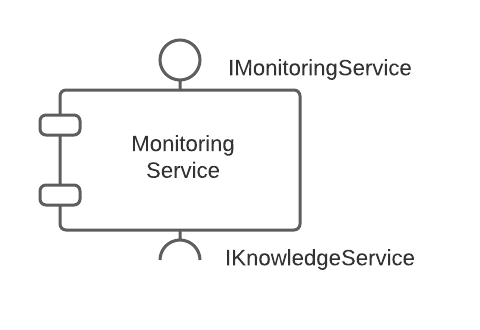
\includegraphics[scale=0.8]{cap_contexto_tecnologico/images/componente-ejemplo}
  \caption{El servicio de monitorización representado como un componente. Ofrece una interfaz (\emph{IMonitoringService}) y depende de otra para funcionar (\emph{IKnowledgeService}).}
  \label{fig:componenteEjemplo}
\end{wrapfigure}

Los componentes exponen una \textbf{interfaz} que permite acceder a la funcionalidad o datos que encapsulan. A su vez, también declaran una serie de \textbf{dependencias} con interfaces de otros. Allí se incluyen todos los elementos que requieren para poder funcionar. En la figura \ref{fig:componenteEjemplo} tenemos un ejemplo. \emph{Monitoring Service} expone la interfaz \emph{IMonitoringService}. Para poder funcionar, depende de un componente que ofrezca \emph{IKnowledgeService}.

Por si solos, estos componentes independientes no aportan mucho valor. Más bien son la unidad básica de composición: podemos combinar varios de ellos para que trabajen conjuntamente y realicen tareas más complejas. Así, podemos \textbf{componer sistemas}. \cite{mehtaTaxonomySoftwareConnectors2000} La integración y la interacción entre ellos son aspectos clave que debemos abordar.

\subsubsection{Conectores}

Para que dos o más componentes puedan interactuar, necesitamos definir un mecanismo de comunicación. Recurrimos entonces a los \textbf{conectores}. Se trata de elementos arquitectónicos que nos ayudan a definir y razonar sobre la comunicación entre componentes. En la figura \ref{fig:componentesYConectorEjemplo} mostramos una representación de la necesidad de comunicación entre dos componentes a través de un conector. No se ha especificado todavía ningún detalle sobre cómo se implementará. Así, podemos estudiar la arquitectura y elegir los mecanismos adecuados para cada interacción del sistema. \cite{taylorSoftwareArchitectureFoundations2009}.

%% TODO: Los conectores son application-independent. No dependen de la funcionalidad de la aplicación.
%% TODO: Hablar de la cardinalidad de los conectores.

\begin{figure}[h!]
  \centering
  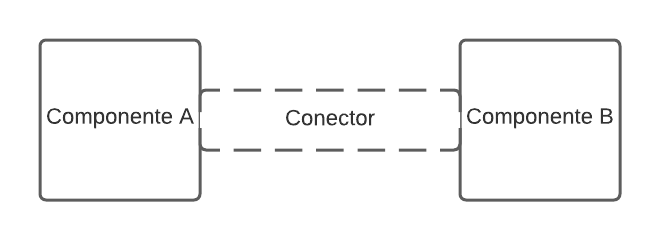
\includegraphics[scale=0.78]{cap_contexto_tecnologico/images/conector}
  \caption{Ejemplo de comunicación de dos componentes a través de un conector.}
  \label{fig:componentesYConectorEjemplo}
\end{figure}

Internamente, los conectores están compuestos por uno o más \textbf{conductos} o canales. A través de estos se lleva a cabo la comunicación entre los componentes. Hay una gran variedad de conductos posibles: comunicación interproceso, a través de la red, etc. Clasificamos los conectores según la complejidad de los canales que utilizan \cite{mehtaTaxonomySoftwareConnectors2000}:

\begin{itemize}
    \item \textbf{Conectores simples}: solo cuentan con un conducto, sin lógica asociada. Son conectores sencillos. Suelen estar ya implementados en los lenguajes de programación. Por ejemplo: una llamada a función en un programa o el sistema de entrada / salida de ficheros.

    \item \textbf{Conectores complejos}: cuentan con uno o más conductos. Se definen por composición a partir de múltiples conectores simples. Además, pueden contar con funcionalidad para manejar el flujo de datos y/o control. Suelen utilizarse importando \emph{frameworks} o librerias. Por ejemplo: un balanceador de carga que redirige peticiones a los nodos.
\end{itemize}

Por tanto, cuando hayamos decidido que dos componentes necesitan comunicarse, es momento de evaluar qué mecanismo de comunicación es más adecuado. Basándonos en nuestros requisitos, la arquitectura ya definida, y los mecanismos de despliegue que queremos usar, elegimos el conector apropiado. Podemos orientarnos con taxonomías como la de \cite{mehtaTaxonomySoftwareConnectors2000}.

\subsubsection{Estilos arquitectónicos}

\textcolor{red}{TODO: Descripción breve}

\textcolor{red}{Podemos agrupar decisiones principales.}
